\documentclass[12pt]{article}
\usepackage{tikz}
\usetikzlibrary{positioning}
\usetikzlibrary{shadings}

\RequirePackage{xcolor}
\definecolor{IHMEdarkblue}{HTML}{0F7C95}
\definecolor{IHMEmiddleblue}{HTML}{17B9CF}
\definecolor{IHMElightblue}{HTML}{86F3F3}
\definecolor{IHMEdarkgreen}{HTML}{32CA81}
\definecolor{IHMEmiddlegreen}{HTML}{89FFA8}
\definecolor{IHMElightgreen}{HTML}{D4FFDB}
\definecolor{IHMEdarkgrey}{HTML}{9EA0A1}
\definecolor{IHMEmiddlegrey}{HTML}{D6D6D6}
\definecolor{IHMElightgrey}{HTML}{F5F5F5}

\begin{document}
\large
\pagestyle{empty}

% Before raking
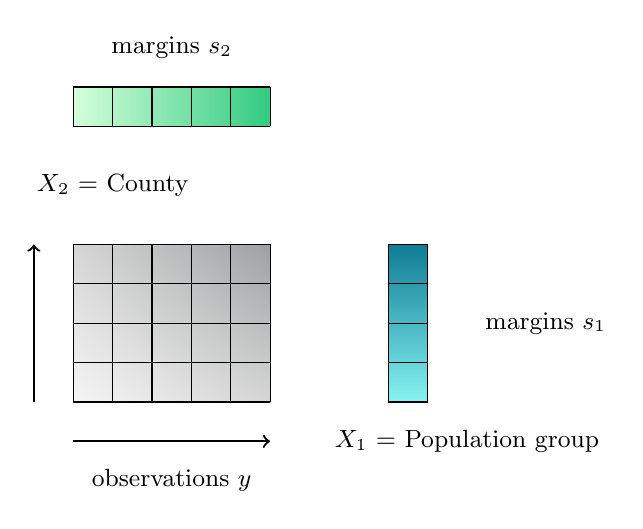
\begin{tikzpicture}[every node/.style={minimum size=0.5cm},on grid]

% Observations
\shade[lower left=IHMElightgrey, upper left=IHMEmiddlegrey, lower right=IHMEmiddlegrey, upper right=IHMEdarkgrey] (0,0) rectangle +(2.5,2.0);
\draw (0,0) grid [step=0.5] (2.5,2.0);

% Margins
\begin{scope}[xshift=4cm]
\shade[top color=IHMEdarkblue, bottom color=IHMElightblue] (0,0) rectangle +(0.5,2.0);
\draw (0,0) grid [step=0.5] (0.5,2.0);
\end{scope}

\begin{scope}[yshift=3.5cm]
\shade[right color=IHMEdarkgreen, left color=IHMElightgreen] (0,0) rectangle +(2.5,0.5);
\draw (0,0) grid [step=0.5] (2.5,0.5);
\end{scope}

\draw (1.25,-1) node[font=\small] {observations $y$};
\draw (6,1.0) node[font=\small] {margins $s_1$};
\draw (1.25,4.5) node[font=\small] {margins $s_2$};

\draw[->,thick] (0,-0.5) -- (2.5,-0.5);
\draw[->,thick] (-0.5,0) -- (-0.5,2.0);

\draw (5,-0.5) node[font=\small] {$X_1$ = Population group};
\draw (0.5,2.75) node[font=\small] {$X_2$ = County};

\end{tikzpicture}

\end{document}

